\documentclass[aspectratio=169]{beamer}

% -------------------------
% Basic packages
% -------------------------
\usepackage[utf8]{inputenc}
\usepackage{graphicx}
\usepackage{amsmath, amssymb}
\usepackage{booktabs}
\usepackage{array}
\usepackage{tikz}
\usepackage{tcolorbox}
\usepackage{hyperref}
\definecolor{questionbg}{RGB}{235, 244, 255}
\definecolor{questionframe}{RGB}{44, 95, 173}
\definecolor{plainbg}{RGB}{241, 249, 241}
\definecolor{plainframe}{RGB}{44, 122, 70}
\definecolor{notationbg}{RGB}{255, 248, 230}
\definecolor{notationframe}{RGB}{176, 118, 0}

\newtcolorbox{questionbox}{
  colback=questionbg,
  colframe=questionframe,
  boxrule=0.7pt,
  arc=1mm,
  fontupper=\small,
  left=1mm,
  right=1mm,
  top=0.4mm,
  bottom=0.4mm
}

\newtcolorbox{plainbox}{
  colback=plainbg,
  colframe=plainframe,
  boxrule=0.7pt,
  arc=1mm,
  fontupper=\small,
  left=1mm,
  right=1mm,
  top=0.4mm,
  bottom=0.4mm
}

\newtcolorbox{notationbox}{
  colback=notationbg,
  colframe=notationframe,
  boxrule=0.7pt,
  arc=1mm,
  fontupper=\small,
  left=1mm,
  right=1mm,
  top=0.4mm,
  bottom=0.4mm
}

\newcommand{\keyquestion}[1]{%
  \begin{questionbox}
  \textbf{Question:} #1
  \end{questionbox}
}

\newcommand{\plainidea}[1]{%
  \begin{plainbox}
  \textbf{Main idea:} #1
  \end{plainbox}
}

\newcommand{\notationblock}[1]{%
  \begin{notationbox}
  \textbf{Symbols used on this slide}\\
  #1
  \end{notationbox}
}

\newcommand{\exercisebreakcontent}[1]{%
  \begin{center}
  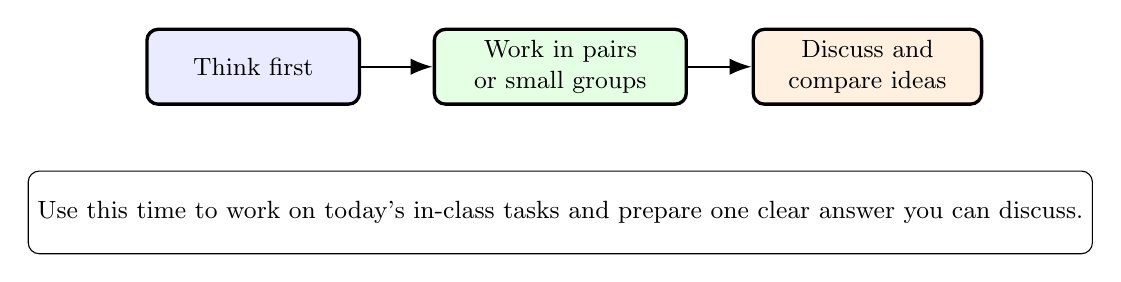
\begin{tikzpicture}[>=Latex, every node/.style={font=\small}]
    \node[draw, rounded corners, very thick, fill=blue!8, minimum width=2.7cm, minimum height=0.95cm, align=center] (think) at (-3.9,0.9) {Think first};
    \node[draw, rounded corners, very thick, fill=green!10, minimum width=3.2cm, minimum height=0.95cm, align=center] (work) at (0,0.9) {Work in pairs\\or small groups};
    \node[draw, rounded corners, very thick, fill=orange!12, minimum width=2.9cm, minimum height=0.95cm, align=center] (share) at (3.9,0.9) {Discuss and\\compare ideas};
    \draw[-{Latex[length=2.8mm]}, thick] (think) -- (work);
    \draw[-{Latex[length=2.8mm]}, thick] (work) -- (share);
    \node[draw, rounded corners, fill=white, minimum width=9.4cm, minimum height=1.05cm, align=center] at (0,-0.95) {Use this time to work on today's in-class tasks and prepare one clear answer you can discuss.};
  \end{tikzpicture}
  \end{center}
  \plainidea{#1}
}

\usetikzlibrary{positioning,arrows.meta,fit,calc}

% -------------------------
% Theme
% -------------------------
\usetheme{Madrid}
\usecolortheme{default}
\setbeamertemplate{navigation symbols}{}

% -------------------------
% Per-slide reference footer
% -------------------------
\newcommand{\defaultdeckrefs}{AIMA4e Ch.13 pp.412--460; Poole3e Ch.9 pp.375--458}
\newcommand{\currentsliderefs}{\defaultdeckrefs}
\newcommand{\setslideref}[1]{\gdef\currentsliderefs{#1}}
\addtobeamertemplate{footline}{}{%
  \begin{beamercolorbox}[wd=\paperwidth,leftskip=0.4em,rightskip=0.4em,ht=2.8ex,dp=0.9ex]{author in head/foot}
    \tiny\textbf{Refs: }\currentsliderefs
  \end{beamercolorbox}
}

% -------------------------
% Metadata
% -------------------------
\title[EBU6505 B4 D2]{EBU6505 -- Reasoning and Agents\\Block 4, Day 2 -- Exact Inference in Bayesian Networks}
\author{Dr Riasat Islam}
\institute{Queen Mary University of London}
\date{}

% -------------------------
% TikZ styles
% -------------------------
\tikzset{
  flowarrow/.style={-{Latex[length=2.8mm]}, thick},
  softarrow/.style={-{Latex[length=2.4mm]}, thick, gray!70},
  bnnode/.style={draw, rounded corners, very thick, fill=blue!8, minimum width=2.2cm, minimum height=0.95cm, align=center},
  querynode/.style={draw, rounded corners, very thick, fill=blue!14, minimum width=2.2cm, minimum height=0.95cm, align=center},
  evidnode/.style={draw, rounded corners, very thick, fill=green!14, minimum width=2.2cm, minimum height=0.95cm, align=center},
  hiddennode/.style={draw, rounded corners, very thick, fill=orange!14, minimum width=2.2cm, minimum height=0.95cm, align=center},
  factorbox/.style={draw, rounded corners, very thick, fill=white, minimum width=2.8cm, minimum height=1.0cm, align=center},
  note/.style={draw, rounded corners, fill=white, minimum width=2.9cm, minimum height=0.95cm, align=center},
  relabel/.style={font=\small, fill=white, inner sep=1pt}
}

\begin{document}

\setslideref{AIMA4e Ch.13 pp.412--460; Poole3e Ch.9 pp.375--458}
\begin{frame}
  \titlepage
\end{frame}

\begin{frame}{What have we covered this week?}
\begin{itemize}
  \item Day 1: what a Bayesian network is
  \item nodes, arrows, and CPTs
  \item how the graph encodes conditional independence
  \item how a network represents one joint probability model
\end{itemize}
\plainidea{Yesterday we learned how to read the model. Today we learn how to get an answer from the model.}
\end{frame}

\begin{frame}{What are we going to cover today?}
\begin{itemize}
  \item what an inference query looks like
  \item enumeration as the direct exact method
  \item variable elimination as the smarter exact method
  \item why elimination order and treewidth matter
  \item when exact inference becomes too expensive
\end{itemize}
\plainidea{The whole lecture answers one question: once we have a Bayesian network, how do we use it to compute a probability?}
\end{frame}

\begin{frame}{Resources}
\small
\begin{itemize}
  \item \textit{Artificial Intelligence: A Modern Approach}, Russell and Norvig (4th ed.)
  \item AIMA 4e, Chapter 13: Exact Inference in Bayesian Networks
  \item \textit{Artificial Intelligence: Foundations of Computational Agents}, David Poole and Alan Mackworth (3rd ed.)
  \item Poole 3e, Chapter 9: Probabilistic Inference
\end{itemize}
\plainidea{Both books cover the same two exact methods for today: enumeration and variable elimination.}
\end{frame}

\begin{frame}{Learning Outcomes for Today}
\begin{itemize}
  \item identify the query, evidence, and hidden variables in a BN question
  \item explain enumeration in simple words
  \item explain how variable elimination avoids repeated work
  \item read the meaning of factor product, summing out, and normalisation
  \item explain why exact inference gets harder in more connected graphs
\end{itemize}
\plainidea{If these five ideas are clear, students can follow exact-inference calculations without getting lost in notation.}
\end{frame}

\begin{frame}{Warm-Up Question}
\keyquestion{If John and Mary both call, how do we compute the probability of a burglary?}
\begin{columns}[T,onlytextwidth]
  \begin{column}{0.50\textwidth}
    \begin{center}
    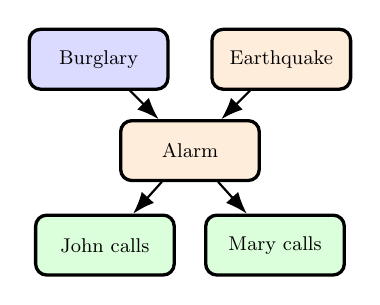
\begin{tikzpicture}[>=Latex, scale=0.80, every node/.style={font=\small, transform shape}]
      \node[querynode] (b) at (0,1.25) {Burglary};
      \node[hiddennode] (e) at (2.9,1.25) {Earthquake};
      \node[hiddennode] (a) at (1.45,-0.2) {Alarm};
      \node[evidnode] (j) at (0.1,-1.7) {John calls};
      \node[evidnode] (m) at (2.8,-1.7) {Mary calls};
      \draw[flowarrow] (b) -- (a);
      \draw[flowarrow] (e) -- (a);
      \draw[flowarrow] (a) -- (j);
      \draw[flowarrow] (a) -- (m);
    \end{tikzpicture}
    \end{center}
  \end{column}
  \begin{column}{0.47\textwidth}
    \begin{tcolorbox}[colback=questionbg,colframe=questionframe,boxrule=0.7pt,title=What is known?]
    We know the graph and the CPTs.\\[0.2em]
    We observe two calls.
    \end{tcolorbox}
    \begin{tcolorbox}[colback=plainbg,colframe=plainframe,boxrule=0.7pt,title=What is unknown?]
    We want the probability of burglary after seeing the calls.
    \end{tcolorbox}
    \[
    P(B \mid J{=}t, M{=}t)
    \]
  \end{column}
\end{columns}
\vspace{-0.25em}
\plainidea{Inference means: use the model plus the evidence to compute the probability of the query variable.}
\end{frame}

\begin{frame}{How Do We Read an Inference Query?}
\keyquestion{Which part is the answer, and which part is the evidence?}
\begin{center}
\[
P(B \mid J{=}t, M{=}t)
\]
\end{center}
\begin{columns}[T,onlytextwidth]
  \begin{column}{0.31\textwidth}
    \begin{tcolorbox}[colback=questionbg,colframe=questionframe,boxrule=0.7pt,title=Query]
    $B$\\
    the variable we want to know about
    \end{tcolorbox}
  \end{column}
  \begin{column}{0.31\textwidth}
    \begin{tcolorbox}[colback=plainbg,colframe=plainframe,boxrule=0.7pt,title=Evidence]
    $J{=}t,\ M{=}t$\\
    the facts we have observed
    \end{tcolorbox}
  \end{column}
  \begin{column}{0.31\textwidth}
    \begin{tcolorbox}[colback=notationbg,colframe=notationframe,boxrule=0.7pt,title=Hidden variables]
    $A,\ E$\\
    not observed, but still relevant
    \end{tcolorbox}
  \end{column}
\end{columns}
\plainidea{A Bayesian-network query always separates into query variables, observed evidence, and hidden variables that must be handled in the calculation.}
\end{frame}

\begin{frame}{Exact or Approximate?}
\keyquestion{What kind of answer do we want today?}
\begin{columns}[T,onlytextwidth]
  \begin{column}{0.48\textwidth}
    \begin{tcolorbox}[colback=plainbg,colframe=plainframe,boxrule=0.7pt,title=Exact inference]
    \begin{itemize}
      \item returns the exact probability
      \item uses full probability calculation
      \item good for small and moderate networks
    \end{itemize}
    \end{tcolorbox}
  \end{column}
  \begin{column}{0.48\textwidth}
    \begin{tcolorbox}[colback=questionbg,colframe=questionframe,boxrule=0.7pt,title=Approximate inference]
    \begin{itemize}
      \item returns an estimate
      \item often uses sampling
      \item helpful when exact inference is too expensive
    \end{itemize}
    \end{tcolorbox}
  \end{column}
\end{columns}
\plainidea{Today we focus on exact inference, so every answer comes from full probability calculation rather than estimation.}
\end{frame}

\begin{frame}{General Goal of Exact Inference}
\keyquestion{What does the exact-inference formula say in plain words?}
\begin{columns}[T,onlytextwidth]
  \begin{column}{0.52\textwidth}
    \[
    P(X \mid e)= \alpha \sum_{y} P(X,e,y)
    \]
    \begin{tcolorbox}[colback=plainbg,colframe=plainframe,boxrule=0.7pt,title=In simple words]
    Keep the query variable.\\
    Hold the evidence fixed.\\
    Add over every hidden possibility.\\
    Then normalise.
    \end{tcolorbox}
  \end{column}
  \begin{column}{0.43\textwidth}
    \notationblock{$X$: query variable\\
    $e$: observed evidence\\
    $y$: hidden variables\\
    $\alpha$: normalisation constant}
  \end{column}
\end{columns}
\plainidea{Exact inference is just controlled summation over the hidden parts of the model.}
\end{frame}

\begin{frame}{Enumeration: The Most Direct Method}
\keyquestion{If we do inference in the simplest possible way, what do we do?}
\begin{center}
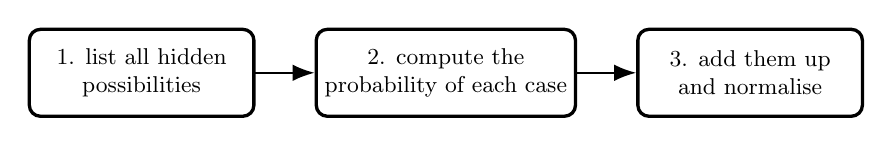
\begin{tikzpicture}[>=Latex, scale=0.92, every node/.style={font=\small, transform shape}]
  \node[factorbox, minimum width=3.1cm, minimum height=1.2cm] (s1) at (0,0) {1. list all hidden\\possibilities};
  \node[factorbox, minimum width=3.1cm, minimum height=1.2cm] (s2) at (4.2,0) {2. compute the\\probability of each case};
  \node[factorbox, minimum width=3.1cm, minimum height=1.2cm] (s3) at (8.4,0) {3. add them up\\and normalise};
  \draw[flowarrow] (s1) -- (s2);
  \draw[flowarrow] (s2) -- (s3);
\end{tikzpicture}
\end{center}
\plainidea{Enumeration is correct and easy to explain, but it can become slow because the number of hidden cases grows quickly.}
\end{frame}

\begin{frame}{Which Variables Are Hidden in the Alarm Query?}
\keyquestion{When we ask about burglary, which variables do we still have to sum over?}
\begin{center}
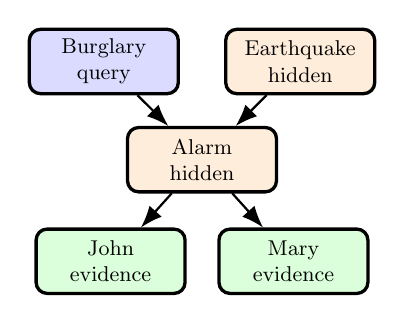
\begin{tikzpicture}[>=Latex, scale=0.86, every node/.style={font=\small, transform shape}]
  \node[querynode] (b) at (0,1.25) {Burglary\\query};
  \node[hiddennode] (e) at (2.9,1.25) {Earthquake\\hidden};
  \node[hiddennode] (a) at (1.45,-0.2) {Alarm\\hidden};
  \node[evidnode] (j) at (0.1,-1.7) {John\\evidence};
  \node[evidnode] (m) at (2.8,-1.7) {Mary\\evidence};
  \draw[flowarrow] (b) -- (a);
  \draw[flowarrow] (e) -- (a);
  \draw[flowarrow] (a) -- (j);
  \draw[flowarrow] (a) -- (m);
\end{tikzpicture}
\end{center}
\plainidea{For this query, the evidence is fixed, the query is Burglary, and the hidden variables are Earthquake and Alarm.}
\end{frame}

\begin{frame}{Write the Enumeration Query}
\keyquestion{What exact expression should we compute for the alarm example?}
\[
P(B \mid j,m)= \alpha \sum_{e}\sum_{a} P(B,e,a,j,m)
\]
\begin{columns}[T,onlytextwidth]
  \begin{column}{0.48\textwidth}
    \begin{tcolorbox}[colback=questionbg,colframe=questionframe,boxrule=0.7pt,title=Why two sums?]
    Earthquake and Alarm are hidden, so we must add over both.
    \end{tcolorbox}
  \end{column}
  \begin{column}{0.48\textwidth}
    \begin{tcolorbox}[colback=plainbg,colframe=plainframe,boxrule=0.7pt,title=What stays fixed?]
    The query variable $B$ and the evidence $j,m$ stay in the expression.
    \end{tcolorbox}
  \end{column}
\end{columns}
\plainidea{Enumeration writes the full query, then sums over the hidden variables.}
\end{frame}

\begin{frame}{Break the Joint into Local Pieces}
\keyquestion{Where does the graph help in the calculation?}
\[
P(B,e,a,j,m)=P(B)\,P(E)\,P(A \mid B,E)\,P(J \mid A)\,P(M \mid A)
\]
\begin{center}
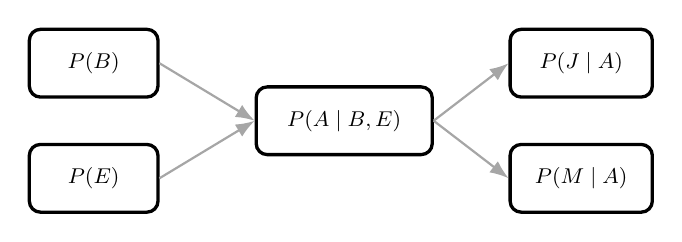
\begin{tikzpicture}[>=Latex, scale=0.86, every node/.style={font=\small, transform shape}]
  \node[factorbox, minimum width=1.9cm] (f1) at (0,0.85) {$P(B)$};
  \node[factorbox, minimum width=1.9cm] (f2) at (0,-0.85) {$P(E)$};
  \node[factorbox, minimum width=2.6cm] (f3) at (3.7,0) {$P(A \mid B,E)$};
  \node[factorbox, minimum width=2.1cm] (f4) at (7.2,0.85) {$P(J \mid A)$};
  \node[factorbox, minimum width=2.1cm] (f5) at (7.2,-0.85) {$P(M \mid A)$};
  \draw[softarrow] (f1.east) -- (f3.west);
  \draw[softarrow] (f2.east) -- (f3.west);
  \draw[softarrow] (f3.east) -- (f4.west);
  \draw[softarrow] (f3.east) -- (f5.west);
\end{tikzpicture}
\end{center}
\plainidea{The graph lets us replace one big joint probability with several small local terms.}
\end{frame}

\begin{frame}{Enumeration Case 1: Assume Burglary Is True}
\keyquestion{What do we do after choosing one value of the query variable?}
\begin{columns}[T,onlytextwidth]
  \begin{column}{0.52\textwidth}
    \[
    \text{score}(B{=}t)= \sum_{e}\sum_{a} P(B{=}t,e,a,j,m)
    \]
    \begin{tcolorbox}[colback=plainbg,colframe=plainframe,boxrule=0.7pt,title=Hidden cases to add]
    $(E{=}t,A{=}t)$,\ $(E{=}t,A{=}f)$,\\
    $(E{=}f,A{=}t)$,\ $(E{=}f,A{=}f)$
    \end{tcolorbox}
  \end{column}
  \begin{column}{0.44\textwidth}
    \begin{center}
    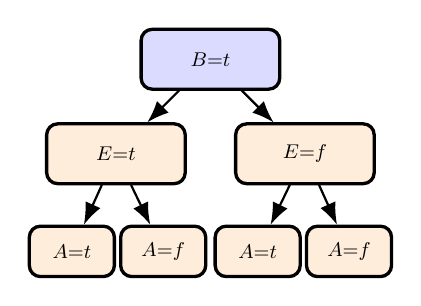
\begin{tikzpicture}[>=Latex, scale=0.80, every node/.style={font=\small, transform shape}]
      \node[querynode] (b) at (0,1.5) {$B{=}t$};
      \node[hiddennode] (e1) at (-1.5,0) {$E{=}t$};
      \node[hiddennode] (e2) at (1.5,0) {$E{=}f$};
      \node[hiddennode, minimum width=1.35cm, minimum height=0.8cm] (a1) at (-2.2,-1.55) {$A{=}t$};
      \node[hiddennode, minimum width=1.35cm, minimum height=0.8cm] (a2) at (-0.75,-1.55) {$A{=}f$};
      \node[hiddennode, minimum width=1.35cm, minimum height=0.8cm] (a3) at (0.75,-1.55) {$A{=}t$};
      \node[hiddennode, minimum width=1.35cm, minimum height=0.8cm] (a4) at (2.2,-1.55) {$A{=}f$};
      \draw[flowarrow] (b) -- (e1);
      \draw[flowarrow] (b) -- (e2);
      \draw[flowarrow] (e1) -- (a1);
      \draw[flowarrow] (e1) -- (a2);
      \draw[flowarrow] (e2) -- (a3);
      \draw[flowarrow] (e2) -- (a4);
    \end{tikzpicture}
    \end{center}
  \end{column}
\end{columns}
\plainidea{For one query value, enumeration adds the probability of every compatible hidden world.}
\end{frame}

\begin{frame}{Enumeration Case 2: Assume Burglary Is False}
\keyquestion{Why do we need a second case for the query variable?}
\begin{columns}[T,onlytextwidth]
  \begin{column}{0.52\textwidth}
    \[
    \text{score}(B{=}f)= \sum_{e}\sum_{a} P(B{=}f,e,a,j,m)
    \]
    \begin{tcolorbox}[colback=questionbg,colframe=questionframe,boxrule=0.7pt,title=Why repeat the process?]
    The final answer is a distribution over $B$, so we need one score for $B{=}t$ and one score for $B{=}f$.
    \end{tcolorbox}
  \end{column}
  \begin{column}{0.44\textwidth}
    \begin{center}
    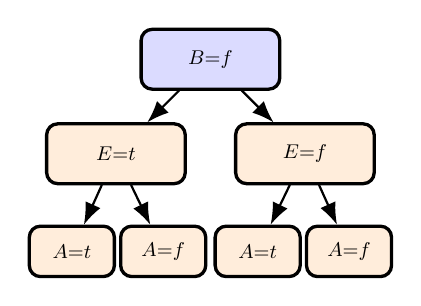
\begin{tikzpicture}[>=Latex, scale=0.80, every node/.style={font=\small, transform shape}]
      \node[querynode] (b) at (0,1.5) {$B{=}f$};
      \node[hiddennode] (e1) at (-1.5,0) {$E{=}t$};
      \node[hiddennode] (e2) at (1.5,0) {$E{=}f$};
      \node[hiddennode, minimum width=1.35cm, minimum height=0.8cm] (a1) at (-2.2,-1.55) {$A{=}t$};
      \node[hiddennode, minimum width=1.35cm, minimum height=0.8cm] (a2) at (-0.75,-1.55) {$A{=}f$};
      \node[hiddennode, minimum width=1.35cm, minimum height=0.8cm] (a3) at (0.75,-1.55) {$A{=}t$};
      \node[hiddennode, minimum width=1.35cm, minimum height=0.8cm] (a4) at (2.2,-1.55) {$A{=}f$};
      \draw[flowarrow] (b) -- (e1);
      \draw[flowarrow] (b) -- (e2);
      \draw[flowarrow] (e1) -- (a1);
      \draw[flowarrow] (e1) -- (a2);
      \draw[flowarrow] (e2) -- (a3);
      \draw[flowarrow] (e2) -- (a4);
    \end{tikzpicture}
    \end{center}
  \end{column}
\end{columns}
\plainidea{Exact inference returns a full normalized distribution, not just one isolated number.}
\end{frame}

\begin{frame}{Normalise the Two Scores}
\keyquestion{How do two unnormalized scores become a valid probability distribution?}
\begin{columns}[T,onlytextwidth]
  \begin{column}{0.48\textwidth}
    \[
    P(B \mid j,m)=
    \frac{\text{score}(B)}
         {\sum_B \text{score}(B)}
    \]
    \begin{tcolorbox}[colback=plainbg,colframe=plainframe,boxrule=0.7pt,title=Result for the alarm example]
    $P(B{=}t \mid j,m) \approx 0.284$\\
    $P(B{=}f \mid j,m) \approx 0.716$
    \end{tcolorbox}
  \end{column}
  \begin{column}{0.48\textwidth}
    \begin{center}
    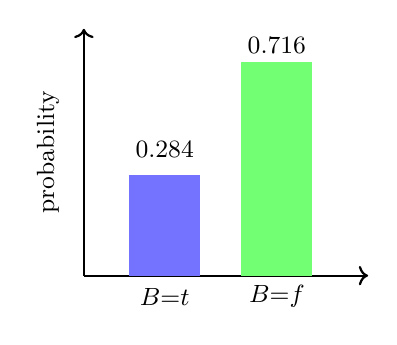
\begin{tikzpicture}[scale=0.95, every node/.style={font=\small}]
      \draw[->, thick] (0,0) -- (0,3.3);
      \draw[->, thick] (0,0) -- (3.8,0);
      \fill[blue!55] (0.6,0) rectangle (1.55,1.35);
      \fill[green!55] (2.1,0) rectangle (3.05,2.85);
      \node at (1.08,-0.28) {$B{=}t$};
      \node at (2.58,-0.28) {$B{=}f$};
      \node[rotate=90] at (-0.48,1.65) {probability};
      \node at (1.08,1.68) {0.284};
      \node at (2.58,3.08) {0.716};
    \end{tikzpicture}
    \end{center}
  \end{column}
\end{columns}
\plainidea{Normalisation rescales the scores so they add up to 1 and become a proper probability distribution.}
\end{frame}

\begin{frame}{In-Class Checkpoint}
\keyquestion{If we observe John and Mary, which variables are evidence and which are hidden?}
\begin{columns}[T,onlytextwidth]
  \begin{column}{0.58\textwidth}
    \begin{tcolorbox}[colback=questionbg,colframe=questionframe,boxrule=0.7pt,title=Discuss with a partner]
    \begin{itemize}
      \item identify the query variable
      \item identify the evidence variables
      \item identify the hidden variables
      \item explain why enumeration needs summation
    \end{itemize}
    \end{tcolorbox}
  \end{column}
  \begin{column}{0.38\textwidth}
    \begin{tcolorbox}[colback=plainbg,colframe=plainframe,boxrule=0.7pt,title=Expected answer]
    Query: $B$\\
    Evidence: $J,M$\\
    Hidden: $A,E$
    \end{tcolorbox}
  \end{column}
\end{columns}
\plainidea{Students should be able to say what is known, what is unknown, and what must be summed over before moving on.}
\end{frame}

\begin{frame}{Why Is Enumeration Wasteful?}
\keyquestion{Where does enumeration waste time?}
\begin{center}
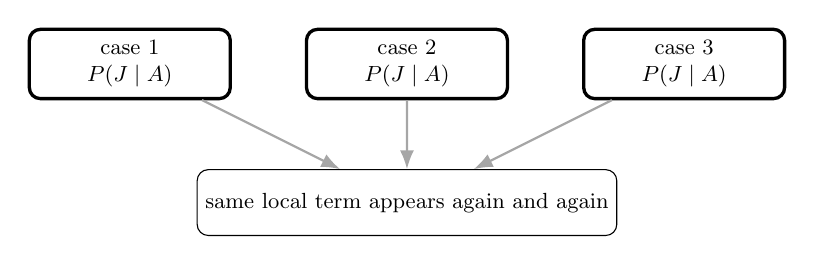
\begin{tikzpicture}[>=Latex, scale=0.88, every node/.style={font=\small, transform shape}]
  \node[factorbox, minimum width=2.9cm] (c1) at (0,0.9) {case 1\\$P(J \mid A)$};
  \node[factorbox, minimum width=2.9cm] (c2) at (4.0,0.9) {case 2\\$P(J \mid A)$};
  \node[factorbox, minimum width=2.9cm] (c3) at (8.0,0.9) {case 3\\$P(J \mid A)$};
  \node[note, minimum width=3.4cm] (rep) at (4.0,-1.1) {same local term appears again and again};
  \draw[softarrow] (c1) -- (rep);
  \draw[softarrow] (c2) -- (rep);
  \draw[softarrow] (c3) -- (rep);
\end{tikzpicture}
\end{center}
\begin{tcolorbox}[colback=questionbg,colframe=questionframe,boxrule=0.7pt]
Enumeration recomputes many of the same local pieces in different hidden cases.
\end{tcolorbox}
\plainidea{Variable elimination is useful because it stores shared intermediate work instead of repeating it.}
\end{frame}

\begin{frame}{Variable Elimination: The Smarter Exact Method}
\keyquestion{How can we stay exact but avoid repeated work?}
\begin{center}
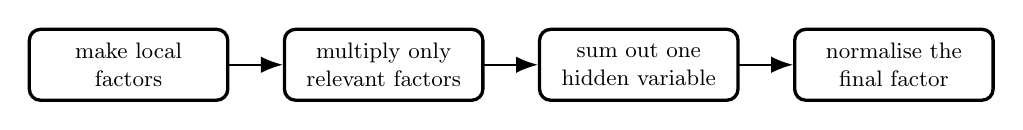
\begin{tikzpicture}[>=Latex, scale=0.9, every node/.style={font=\small, transform shape}]
  \node[factorbox, minimum width=2.8cm] (f1) at (0,0) {make local\\factors};
  \node[factorbox, minimum width=2.8cm] (f2) at (3.6,0) {multiply only\\relevant factors};
  \node[factorbox, minimum width=2.8cm] (f3) at (7.2,0) {sum out one\\hidden variable};
  \node[factorbox, minimum width=2.8cm] (f4) at (10.8,0) {normalise the\\final factor};
  \draw[flowarrow] (f1) -- (f2);
  \draw[flowarrow] (f2) -- (f3);
  \draw[flowarrow] (f3) -- (f4);
\end{tikzpicture}
\end{center}
\plainidea{Variable elimination is still exact, but it organises the work so common pieces are reused.}
\end{frame}

\begin{frame}{What Is a Factor?}
\keyquestion{What object does variable elimination work with?}
\begin{columns}[T,onlytextwidth]
  \begin{column}{0.46\textwidth}
    \begin{center}
    \begin{tabular}{lcc}
    \toprule
    $A$ & $P(J{=}t \mid A)$ \\
    \midrule
    $t$ & 0.90 \\
    $f$ & 0.05 \\
    \bottomrule
    \end{tabular}
    \end{center}
  \end{column}
  \begin{column}{0.50\textwidth}
    \begin{tcolorbox}[colback=plainbg,colframe=plainframe,boxrule=0.7pt,title=Simple meaning]
    A factor is just a small table that stores numbers for some variables.
    \end{tcolorbox}
    \begin{tcolorbox}[colback=notationbg,colframe=notationframe,boxrule=0.7pt,title=Example]
    After applying evidence, a CPT can become a factor over fewer variables.
    \end{tcolorbox}
  \end{column}
\end{columns}
\plainidea{Variable elimination works with small tables called factors, not with one giant joint table.}
\end{frame}

\begin{frame}{Two Operations Drive Variable Elimination}
\keyquestion{What are the only two operations we really need?}
\begin{columns}[T,onlytextwidth]
  \begin{column}{0.48\textwidth}
    \begin{tcolorbox}[colback=questionbg,colframe=questionframe,boxrule=0.7pt,title=1. Pointwise product]
    line up matching rows and multiply the numbers
    \[
    f(A,B)\times g(B,C)
    \]
    \end{tcolorbox}
  \end{column}
  \begin{column}{0.48\textwidth}
    \begin{tcolorbox}[colback=plainbg,colframe=plainframe,boxrule=0.7pt,title=2. Summing out]
    remove a hidden variable by adding over its values
    \[
    \sum_{A} h(A,B,E)
    \]
    \end{tcolorbox}
  \end{column}
\end{columns}
\plainidea{VE keeps combining useful factors and then removing hidden variables one at a time.}
\end{frame}

\begin{frame}{What Does Pointwise Product Mean?}
\keyquestion{How do two small factors become one larger factor?}
\begin{columns}[T,onlytextwidth]
  \begin{column}{0.50\textwidth}
    \[
    f(A,B)\times g(B,C)=h(A,B,C)
    \]
    \begin{tcolorbox}[colback=plainbg,colframe=plainframe,boxrule=0.7pt,title=How to think about it]
    Keep the shared variable aligned. Multiply row by row. The result remembers all variables that still matter.
    \end{tcolorbox}
  \end{column}
  \begin{column}{0.46\textwidth}
    \begin{center}
    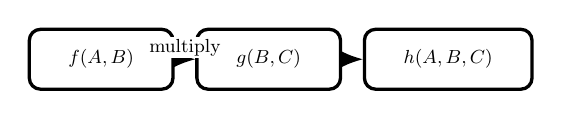
\begin{tikzpicture}[>=Latex, scale=0.76, every node/.style={font=\small, transform shape}]
      \node[factorbox, minimum width=2.4cm] (f) at (0,0) {$f(A,B)$};
      \node[factorbox, minimum width=2.4cm] (g) at (2.8,0) {$g(B,C)$};
      \node[factorbox, minimum width=2.8cm] (h) at (5.8,0) {$h(A,B,C)$};
      \draw[flowarrow] (f) -- node[relabel, above] {multiply} (g);
      \draw[flowarrow] (g) -- (h);
    \end{tikzpicture}
    \end{center}
  \end{column}
\end{columns}
\plainidea{Pointwise product combines local information into one shared factor.}
\end{frame}

\begin{frame}{What Does Summing Out Mean?}
\keyquestion{How do we remove a hidden variable after using it?}
\begin{columns}[T,onlytextwidth]
  \begin{column}{0.50\textwidth}
    \[
    h(B,E)= \sum_{A} f(A,B,E)
    \]
    \begin{tcolorbox}[colback=questionbg,colframe=questionframe,boxrule=0.7pt,title=Plain meaning]
    After variable $A$ has done its job, add over its values and keep only the variables we still need.
    \end{tcolorbox}
  \end{column}
  \begin{column}{0.46\textwidth}
    \begin{center}
    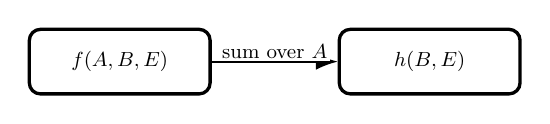
\begin{tikzpicture}[>=Latex, scale=0.82, every node/.style={font=\small, transform shape}]
      \node[factorbox, minimum width=2.8cm] (f) at (0,0) {$f(A,B,E)$};
      \node[factorbox, minimum width=2.8cm] (h) at (4.8,0) {$h(B,E)$};
      \draw[flowarrow] (f) -- node[relabel, above] {sum over $A$} (h);
    \end{tikzpicture}
    \end{center}
  \end{column}
\end{columns}
\plainidea{Summing out removes one hidden variable while preserving its overall effect on the remaining variables.}
\end{frame}

\begin{frame}{Variable Elimination Workflow for the Alarm Query}
\keyquestion{What is the overall plan for this query?}
\begin{center}
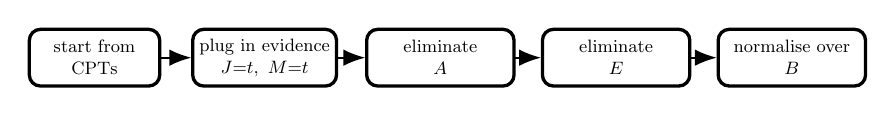
\begin{tikzpicture}[>=Latex, scale=0.72, every node/.style={font=\small, transform shape}]
  \node[factorbox, minimum width=2.3cm] (cpt) at (0,0) {start from\\CPTs};
  \node[factorbox, minimum width=2.5cm] (ev) at (3.0,0) {plug in evidence\\$J{=}t,\ M{=}t$};
  \node[factorbox, minimum width=2.6cm] (a) at (6.1,0) {eliminate\\$A$};
  \node[factorbox, minimum width=2.6cm] (e) at (9.2,0) {eliminate\\$E$};
  \node[factorbox, minimum width=2.6cm] (n) at (12.3,0) {normalise over\\$B$};
  \draw[flowarrow] (cpt) -- (ev);
  \draw[flowarrow] (ev) -- (a);
  \draw[flowarrow] (a) -- (e);
  \draw[flowarrow] (e) -- (n);
\end{tikzpicture}
\end{center}
\plainidea{VE chooses an order for the hidden variables, removes them one by one, and leaves a final factor for the query variable.}
\end{frame}

\begin{frame}{Step 1: Build the Initial Factors}
\keyquestion{What factors do we start with for the alarm network?}
\[
\begin{aligned}
f_1(B) &= P(B) \\
f_2(E) &= P(E) \\
f_3(A,B,E) &= P(A \mid B,E) \\
f_4(J,A) &= P(J \mid A) \\
f_5(M,A) &= P(M \mid A)
\end{aligned}
\]
\begin{tcolorbox}[colback=plainbg,colframe=plainframe,boxrule=0.7pt]
Each factor comes directly from one local CPT in the network.
\end{tcolorbox}
\plainidea{The graph tells us exactly which local factors exist before any evidence is applied.}
\end{frame}

\begin{frame}{Step 2: Apply the Evidence}
\keyquestion{How do the call observations simplify the factors?}
\begin{columns}[T,onlytextwidth]
  \begin{column}{0.52\textwidth}
    \[
    J{=}t,\quad M{=}t
    \]
    \[
    f_4'(A)=P(J{=}t \mid A),\qquad
    f_5'(A)=P(M{=}t \mid A)
    \]
    \begin{tcolorbox}[colback=questionbg,colframe=questionframe,boxrule=0.7pt,title=What changed?]
    The observed variables disappear from the factor arguments because their values are now fixed.
    \end{tcolorbox}
  \end{column}
  \begin{column}{0.44\textwidth}
    \begin{center}
    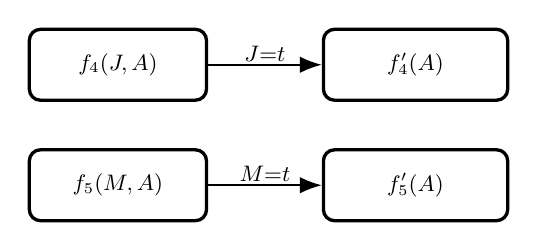
\begin{tikzpicture}[>=Latex, scale=0.9, every node/.style={font=\small, transform shape}]
      \node[factorbox, minimum width=2.5cm] (j1) at (0,0.85) {$f_4(J,A)$};
      \node[factorbox, minimum width=2.5cm] (m1) at (0,-0.85) {$f_5(M,A)$};
      \node[factorbox, minimum width=2.6cm] (j2) at (4.2,0.85) {$f_4'(A)$};
      \node[factorbox, minimum width=2.6cm] (m2) at (4.2,-0.85) {$f_5'(A)$};
      \draw[flowarrow] (j1) -- node[relabel, above] {$J{=}t$} (j2);
      \draw[flowarrow] (m1) -- node[relabel, above] {$M{=}t$} (m2);
    \end{tikzpicture}
    \end{center}
  \end{column}
\end{columns}
\plainidea{Evidence reduces the size of some factors before elimination begins.}
\end{frame}

\begin{frame}{Step 3: Eliminate Alarm}
\keyquestion{What do we do with the first hidden variable?}
\begin{columns}[T,onlytextwidth]
  \begin{column}{0.54\textwidth}
    \[
    f_6(A,B,E)= f_3(A,B,E)\,f_4'(A)\,f_5'(A)
    \]
    \[
    f_7(B,E)= \sum_A f_6(A,B,E)
    \]
    \begin{tcolorbox}[colback=plainbg,colframe=plainframe,boxrule=0.7pt,title=Meaning]
    \raggedright Multiply the three factors that mention $A$. Then sum over $A$ to remove it.
    \end{tcolorbox}
  \end{column}
  \begin{column}{0.42\textwidth}
    \begin{center}
    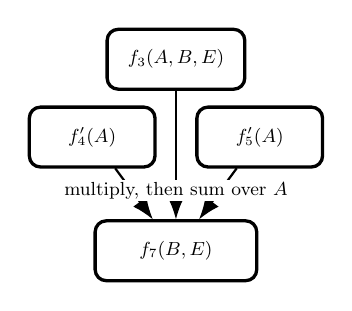
\begin{tikzpicture}[>=Latex, scale=0.76, every node/.style={font=\small, transform shape}]
      \node[factorbox, minimum width=2.3cm] (f3) at (0,1.2) {$f_3(A,B,E)$};
      \node[factorbox, minimum width=2.1cm] (f4) at (-1.4,-0.1) {$f_4'(A)$};
      \node[factorbox, minimum width=2.1cm] (f5) at (1.4,-0.1) {$f_5'(A)$};
      \node[factorbox, minimum width=2.7cm] (f7) at (0,-2.0) {$f_7(B,E)$};
      \draw[flowarrow] (f3) -- (f7);
      \draw[flowarrow] (f4) -- (f7);
      \draw[flowarrow] (f5) -- (f7);
      \node[relabel] at (0,-1.0) {multiply, then sum over $A$};
    \end{tikzpicture}
    \end{center}
  \end{column}
\end{columns}
\plainidea{After using Alarm, keep a smaller factor over $B$ and $E$.}
\end{frame}

\begin{frame}{Step 4: Eliminate Earthquake}
\keyquestion{What is left after Alarm has been removed?}
\begin{columns}[T,onlytextwidth]
  \begin{column}{0.54\textwidth}
    \[
    f_8(B,E)= f_1(B)\,f_2(E)\,f_7(B,E)
    \]
    \[
    f_9(B)= \sum_E f_8(B,E)
    \]
    \begin{tcolorbox}[colback=questionbg,colframe=questionframe,boxrule=0.7pt,title=What remains now?]
    Only the query variable $B$ remains, so we are almost finished.
    \end{tcolorbox}
  \end{column}
  \begin{column}{0.42\textwidth}
    \begin{center}
    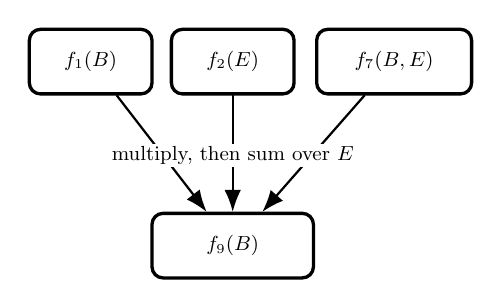
\begin{tikzpicture}[>=Latex, scale=0.82, every node/.style={font=\small, transform shape}]
      \node[factorbox, minimum width=1.9cm] (f1) at (-2.2,1.25) {$f_1(B)$};
      \node[factorbox, minimum width=1.9cm] (f2) at (0,1.25) {$f_2(E)$};
      \node[factorbox, minimum width=2.4cm] (f7) at (2.5,1.25) {$f_7(B,E)$};
      \node[factorbox, minimum width=2.5cm] (f9) at (0,-1.6) {$f_9(B)$};
      \draw[flowarrow] (f1) -- (f9);
      \draw[flowarrow] (f2) -- (f9);
      \draw[flowarrow] (f7) -- (f9);
      \node[relabel] at (0,-0.2) {multiply, then sum over $E$};
    \end{tikzpicture}
    \end{center}
  \end{column}
\end{columns}
\plainidea{VE removes the hidden variables one by one until only the query variable is left.}
\end{frame}

\begin{frame}{Step 5: Normalise the Final Factor}
\keyquestion{Why is the last factor not yet the final answer?}
\begin{columns}[T,onlytextwidth]
  \begin{column}{0.49\textwidth}
    \[
    P(B \mid J{=}t,M{=}t)=
    \frac{f_9(B)}
         {\sum_B f_9(B)}
    \]
    \begin{tcolorbox}[colback=plainbg,colframe=plainframe,boxrule=0.7pt,title=Final answer]
    $P(B{=}t \mid j,m)\approx 0.284$\\
    $P(B{=}f \mid j,m)\approx 0.716$
    \end{tcolorbox}
  \end{column}
  \begin{column}{0.47\textwidth}
    \begin{center}
    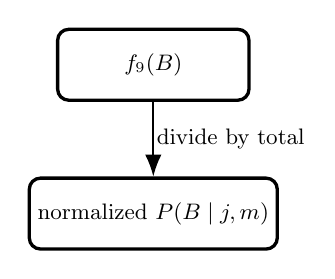
\begin{tikzpicture}[>=Latex, scale=0.9, every node/.style={font=\small, transform shape}]
      \node[factorbox, minimum width=2.7cm] (u) at (0,1.0) {$f_9(B)$};
      \node[factorbox, minimum width=3.3cm] (n) at (0,-1.1) {normalized $P(B \mid j,m)$};
      \draw[flowarrow] (u) -- node[relabel, right] {divide by total} (n);
    \end{tikzpicture}
    \end{center}
  \end{column}
\end{columns}
\plainidea{Normalisation is the last step in both enumeration and variable elimination.}
\end{frame}

\begin{frame}{Why Is Variable Elimination Better Than Enumeration?}
\keyquestion{What work does VE save?}
\begin{columns}[T,onlytextwidth]
  \begin{column}{0.48\textwidth}
    \begin{tcolorbox}[colback=questionbg,colframe=questionframe,boxrule=0.7pt,title=Enumeration]
    \begin{itemize}
      \item lists many hidden cases
      \item repeats local calculations
      \item conceptually simple
    \end{itemize}
    \end{tcolorbox}
  \end{column}
  \begin{column}{0.48\textwidth}
    \begin{tcolorbox}[colback=plainbg,colframe=plainframe,boxrule=0.7pt,title=Variable elimination]
    \begin{itemize}
      \item stores intermediate factors
      \item reuses shared work
      \item often much faster
    \end{itemize}
    \end{tcolorbox}
  \end{column}
\end{columns}
\plainidea{Both methods are exact, but VE is usually preferred because it avoids repeated computation.}
\end{frame}

\begin{frame}{Does Elimination Order Matter?}
\keyquestion{Can the same query become easier or harder depending on the order?}
\begin{columns}[T,onlytextwidth]
  \begin{column}{0.48\textwidth}
    \begin{tcolorbox}[colback=plainbg,colframe=plainframe,boxrule=0.7pt,title=Good order]
    remove a lower-impact variable first\\
    smaller factors
    \end{tcolorbox}
  \end{column}
  \begin{column}{0.48\textwidth}
    \begin{tcolorbox}[colback=questionbg,colframe=questionframe,boxrule=0.7pt,title=Bad order]
    remove a highly connected variable early\\
    larger factors
    \end{tcolorbox}
  \end{column}
\end{columns}
\begin{center}
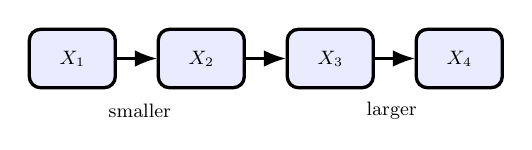
\begin{tikzpicture}[>=Latex, scale=0.78, every node/.style={font=\small, transform shape}]
  \node[bnnode, minimum width=1.4cm] (x1) at (0,0.1) {$X_1$};
  \node[bnnode, minimum width=1.4cm] (x2) at (2.1,0.1) {$X_2$};
  \node[bnnode, minimum width=1.4cm] (x3) at (4.2,0.1) {$X_3$};
  \node[bnnode, minimum width=1.4cm] (x4) at (6.3,0.1) {$X_4$};
  \draw[flowarrow] (x1) -- (x2);
  \draw[flowarrow] (x2) -- (x3);
  \draw[flowarrow] (x3) -- (x4);
  \node[relabel] at (1.1,-0.75) {smaller};
  \node[relabel] at (5.2,-0.75) {larger};
\end{tikzpicture}
\end{center}
\vspace{-0.15em}
\plainidea{Elimination order matters because it changes factor size and cost.}
\end{frame}

\setslideref{AIMA4e Ch.13 pp.412--460; Poole3e Ch.12 pp.517--582}
\begin{frame}{What Is Treewidth in Simple Words?}
\keyquestion{What tells us whether exact inference will stay manageable?}
\begin{columns}[T,onlytextwidth]
  \begin{column}{0.50\textwidth}
    \begin{tcolorbox}[colback=plainbg,colframe=plainframe,boxrule=0.7pt,title=Simple intuition]
    Treewidth asks: what is the biggest group of variables we must keep together inside one intermediate factor?
    \end{tcolorbox}
    \[
    \text{treewidth} \approx \text{largest group size} - 1
    \]
  \end{column}
  \begin{column}{0.45\textwidth}
    \begin{center}
    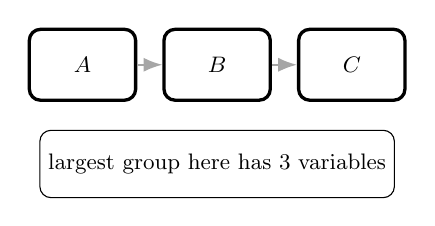
\begin{tikzpicture}[>=Latex, scale=0.9, every node/.style={font=\small, transform shape}]
      \node[factorbox, minimum width=1.5cm] (a) at (0,0) {$A$};
      \node[factorbox, minimum width=1.5cm] (b) at (1.9,0) {$B$};
      \node[factorbox, minimum width=1.5cm] (c) at (3.8,0) {$C$};
      \node[note, minimum width=3.4cm] at (1.9,-1.4) {largest group here has 3 variables};
      \draw[softarrow] (a) -- (b);
      \draw[softarrow] (b) -- (c);
    \end{tikzpicture}
    \end{center}
  \end{column}
\end{columns}
\plainidea{Exact inference is easier when the biggest factor stays small.}
\end{frame}

\begin{frame}{Sparse Graph or Dense Graph?}
\keyquestion{Which kind of network usually gives easier exact inference?}
\begin{columns}[T,onlytextwidth]
  \begin{column}{0.48\textwidth}
    \begin{center}
    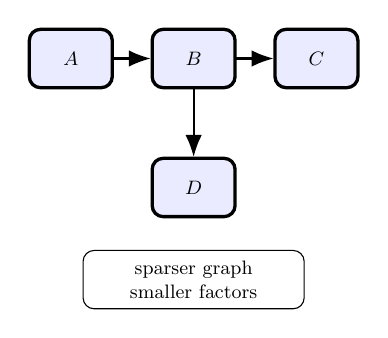
\begin{tikzpicture}[>=Latex, scale=0.78, every node/.style={font=\small, transform shape}]
      \node[bnnode, minimum width=1.35cm] (a) at (0,1.2) {$A$};
      \node[bnnode, minimum width=1.35cm] (b) at (2.0,1.2) {$B$};
      \node[bnnode, minimum width=1.35cm] (c) at (4.0,1.2) {$C$};
      \node[bnnode, minimum width=1.35cm] (d) at (2.0,-0.9) {$D$};
      \draw[flowarrow] (a) -- (b);
      \draw[flowarrow] (b) -- (c);
      \draw[flowarrow] (b) -- (d);
      \node[note, minimum width=3.6cm] at (2.0,-2.4) {sparser graph\\smaller factors};
    \end{tikzpicture}
    \end{center}
  \end{column}
  \begin{column}{0.48\textwidth}
    \begin{center}
    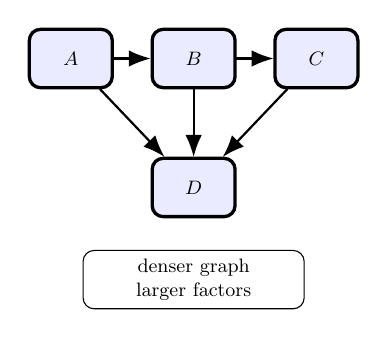
\begin{tikzpicture}[>=Latex, scale=0.78, every node/.style={font=\small, transform shape}]
      \node[bnnode, minimum width=1.35cm] (a) at (0,1.2) {$A$};
      \node[bnnode, minimum width=1.35cm] (b) at (2.0,1.2) {$B$};
      \node[bnnode, minimum width=1.35cm] (c) at (4.0,1.2) {$C$};
      \node[bnnode, minimum width=1.35cm] (d) at (2.0,-0.9) {$D$};
      \draw[flowarrow] (a) -- (b);
      \draw[flowarrow] (b) -- (c);
      \draw[flowarrow] (a) -- (d);
      \draw[flowarrow] (b) -- (d);
      \draw[flowarrow] (c) -- (d);
      \node[note, minimum width=3.6cm] at (2.0,-2.4) {denser graph\\larger factors};
    \end{tikzpicture}
    \end{center}
  \end{column}
\end{columns}
\plainidea{More connections usually mean larger factors and harder exact inference.}
\end{frame}

\begin{frame}{When Does Exact Inference Become Hard?}
\keyquestion{Why can exact inference become too expensive in bigger models?}
\begin{center}
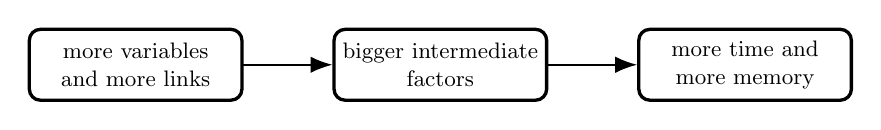
\begin{tikzpicture}[>=Latex, scale=0.9, every node/.style={font=\small, transform shape}]
  \node[factorbox, minimum width=3.0cm] (s1) at (0,0) {more variables\\and more links};
  \node[factorbox, minimum width=3.0cm] (s2) at (4.3,0) {bigger intermediate\\factors};
  \node[factorbox, minimum width=3.0cm] (s3) at (8.6,0) {more time and\\more memory};
  \draw[flowarrow] (s1) -- (s2);
  \draw[flowarrow] (s2) -- (s3);
\end{tikzpicture}
\end{center}
\begin{tcolorbox}[colback=questionbg,colframe=questionframe,boxrule=0.7pt]
This is why exact inference works well on some networks, but not on every realistic large-scale model.
\end{tcolorbox}
\plainidea{The challenge is not the definition of exact inference. The challenge is the size of the intermediate factors it creates.}
\end{frame}

\setslideref{AIMA4e Ch.13--14 pp.412--498; Poole3e Ch.9 pp.375--458}
\begin{frame}{Where Are We Going Next?}
\keyquestion{What changes when uncertainty unfolds over time instead of one static snapshot?}
\begin{columns}[T,onlytextwidth]
  \begin{column}{0.52\textwidth}
    \begin{tcolorbox}[colback=plainbg,colframe=plainframe,boxrule=0.7pt,title=Today]
    one Bayesian network\\
    one fixed inference query
    \end{tcolorbox}
    \begin{tcolorbox}[colback=questionbg,colframe=questionframe,boxrule=0.7pt,title=Next lecture]
    repeated uncertain states across time\\
    state today affects state tomorrow
    \end{tcolorbox}
  \end{column}
  \begin{column}{0.42\textwidth}
    \begin{center}
    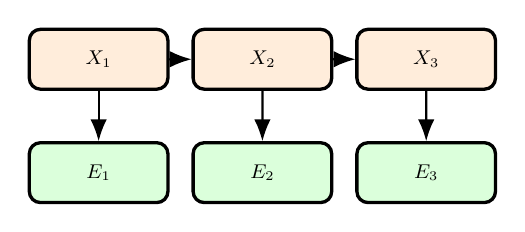
\begin{tikzpicture}[>=Latex, scale=0.80, every node/.style={font=\small, transform shape}]
      \node[hiddennode] (x1) at (0,0.9) {$X_1$};
      \node[evidnode] (e1) at (0,-0.9) {$E_1$};
      \node[hiddennode] (x2) at (2.6,0.9) {$X_2$};
      \node[evidnode] (e2) at (2.6,-0.9) {$E_2$};
      \node[hiddennode] (x3) at (5.2,0.9) {$X_3$};
      \node[evidnode] (e3) at (5.2,-0.9) {$E_3$};
      \draw[flowarrow] (x1) -- (x2);
      \draw[flowarrow] (x2) -- (x3);
      \draw[flowarrow] (x1) -- (e1);
      \draw[flowarrow] (x2) -- (e2);
      \draw[flowarrow] (x3) -- (e3);
    \end{tikzpicture}
    \end{center}
  \end{column}
\end{columns}
\vspace{-0.15em}
\plainidea{Day 3 keeps probabilistic inference but adds time and sequential evidence.}
\end{frame}

\setslideref{AIMA4e Ch.13 pp.412--460; Poole3e Ch.9 pp.375--458}
\begin{frame}{Key Takeaways}
\begin{itemize}
  \item exact inference answers a query using the model plus evidence
  \item enumeration is the direct method: list, multiply, add, normalise
  \item variable elimination is smarter because it reuses intermediate factors
  \item elimination order matters because it changes factor size
  \item treewidth gives an intuition for why exact inference can become hard
\end{itemize}
\plainidea{Students should now see exact inference as a structured workflow, not as a disconnected set of formulas.}
\end{frame}

\begin{frame}{In-Class Exercises}
\exercisebreakcontent{Use the exercise time to explain the inference workflow in clear everyday language, not only in formulas.}
\end{frame}

\begin{frame}{Further Study}
\begin{itemize}
  \item Read Poole Chapter 9 and AIMA Chapter 13.
  \item Practice: Poole Ch.9, Exercises 9.8, 9.9, 9.11, and 9.15.
  \item AIMA Bayesian-network exercise page: 14.18, 14.19, and 14.21.
  \item Focus on enumeration, variable elimination, and why elimination order affects difficulty.
\end{itemize}
\end{frame}

\end{document}
